\chapter{Le détecteur Compact Muon Solenoid (CMS)}
\renewcommand\chapterillustration{CMS/cms.jpeg}
\ThisULCornerWallPaper{1}{\chapterillustration}
\minitoc

\section{Le détecteur Solénoïde compact à muons (CMS)}
Le détecteur Solénoïde compact à muons abrégé en CMS (pour Compact Muon Solenoid) est avec ATLAS une expérience généraliste qui a comme buts majeurs :

\begin{itemize}[label=$\bullet$]
	\item \textbf{La recherche du boson de Higgs : } Lors de la conception de CMS dans les années 1990, la détection du boson de Higgs à été prise comme référence afin de tester les performances du design du détecteur. Ce but à été réalisé avec la découverte d'une particule compatible avec le boson de Higgs le 4 juillet 2012 (cf.\ref{higgs}).
	\begin{figure}[h!]
		\subfloat[Distribution de la masse invariante en mode diphoton, chaque événement étatnt pondéré par S/(s+b) les traits représente le signal et le bruit de fond. Les bandes rpersente les incertitudes décart type $\pm$1 et $\pm 2$ dans l'estimation du bruit de fond.L'encart montre la partie centrale de la distribution de masse invariante non pondérée]{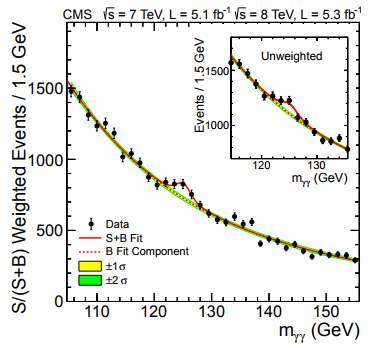
\includegraphics[width=.48\linewidth]{CMS/higgs1.png}}
		\subfloat[Distribution de la masse invariante pour $ZZ\rightarrow 4l$/ Les points représentent les données, l'histogramme plein le bruit de fond et l'histogramme creux le signal pour un boson de Higgs de mass $m_{h}=125$ GeV ajouté au bruit de fond/]{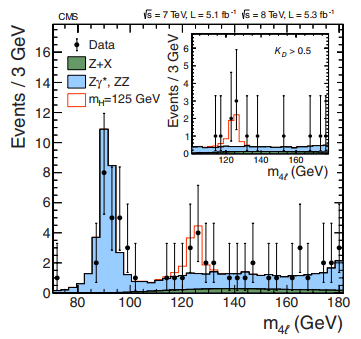
\includegraphics[width=.48\linewidth]{CMS/higgs2.png}}
		\caption{Deux de la masse invariante dans des canaux de désintégration du boson de Higgs montrant sa découverte.[paper]}
		\label{higgs}
	\end{figure}
	\item \textbf{Confirmer et préciser les mesures de la physique du Modèle Standard : } Des mesures de précisions dans des domaines tels que la QCD, le couplage électrofaible, et la physique des saveurs pourrait donner des indications d'une physique au-dlà du Modèle Standard.
	\item \textbf{La recherche de signes de physique au-delà du Modèle Standard : }CMS permet la recherche de particules supersymmétriques ou de nouveaux bosons vecteur massifs ($Z'$) ou encore la recherche de dimensions supplémentaires par exemple.
	\item \textbf{Étudier les collisions d'ions lourds.}
\end{itemize}

Afin de répondre à ses objectifs, le "Technical Design Report" (TDR) a fixé le cahier des charges et les caractéristiques essentielles du détecteur CMS, à savoir :
\begin{itemize}[label=$\bullet$]
	\item Une bonne identification des muons et une bonne résolution en impulssion sur une vaste gamme d'impulssion pour la région $|\eta|<2.5$, une bonne résolution en masse pour les dimuons ($\approx 1\%$ à 100GeV/c$^{2}$) et la capacité à déterminé de manière certaine la charge des muons de $p<$ 1TeV/c.
	\item Une bonne résolution en impulssion pour les particules chargées ainsi qu'une bonne efficacuté de reconstruction dans le trajectographe interne (inner tracker). Un déclenchement et un étiquettage efficace pour les jets venant de quarks $\tau$ et $b$, ce qui requiert un détecteur à pixels proche du point d'interaction.
	\item Une bonne résolution pour l'énergie électromgnétique, et une bonne résolution en masse pour les diphoton et dielectron  ($\approx 1\%$ à 100GeV/c$^{2}$), une grande couverture géométrique ($|\eta|<2.5$), une mesure de la diraction des photons et/ou une correction localisation du vertex primaire d'interaction ainsi qu'une bonne rejection des $\pi_{0}$ et une isolation des photons et letptons efficace à haute luminosité.
	\item une bonne résolution en masse des dijets et une bonne résolution en masse de l'énergie transverse manquante $E_{T}^{miss}$. Ceci requiert un calorimètre hadronique hermétique de très grande couverture géométrique ($|\eta|<5$) et une fine segmentation latérale ($\Delta\nu\times\Delta\Psi<0.1\times0.1$)
\end{itemize} 

\subsection{Description générale de CMS}
Le détécteur CMS se trouve dans une caverne situé au point 5 (P5), proche du village de Cessy en France. La construction de CMS s'est effectué en surface et par tranches autonomes afin de réduire le temps et les coûts nécessaire à sa construction. Chaque tranche à ensuite été descendu dans la caverne et assemblé à 100 m sous terre (cf.fig\ref{slice}).
\marginpar
{
	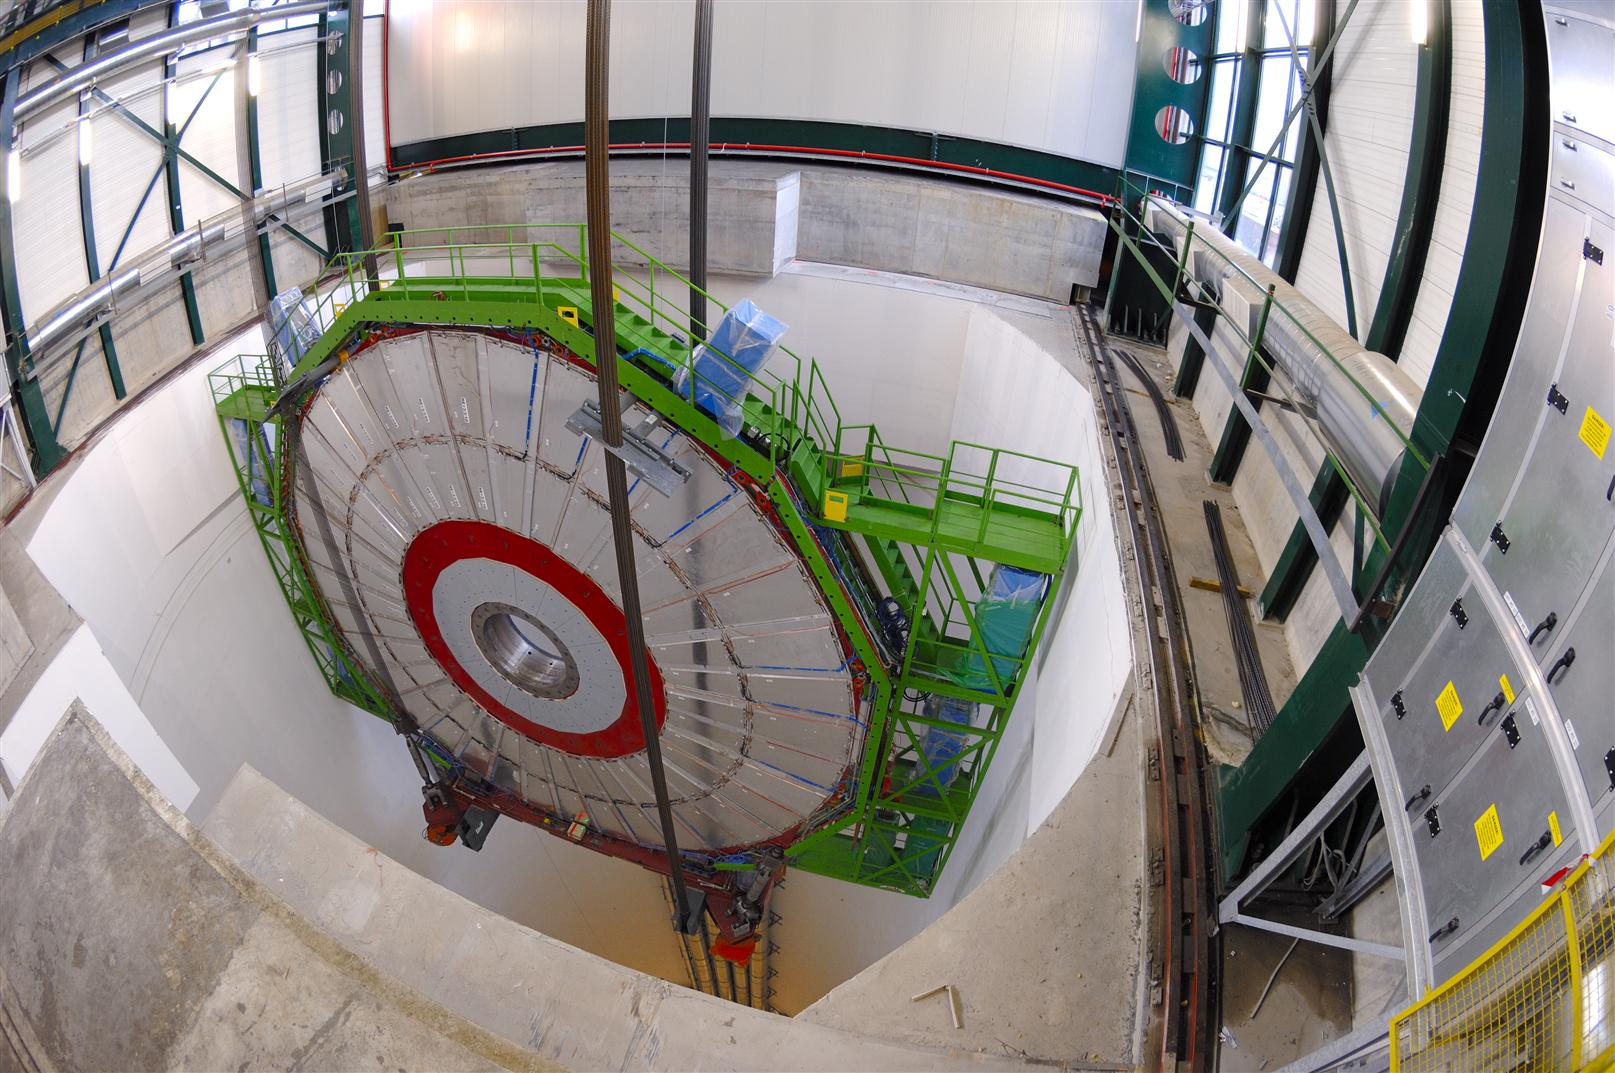
\includegraphics[width=\marginparwidth]{CMS/slice.jpg}
	\captionof{figure}{Descente d'unr tranche de CMS dans la caverne au point P5.}
	\label{slice}
}

CMS est une détecteur cylindrique de 24m de long et de 14.6 m de diamètre pour une masse de plus de 16000 tonnes (cf.fig\ref{cmsexploded}). Le design de CMS est motivé par la mesure de l'impulsion transverse des 

\begin{sidewaysfigure}
	\centering
	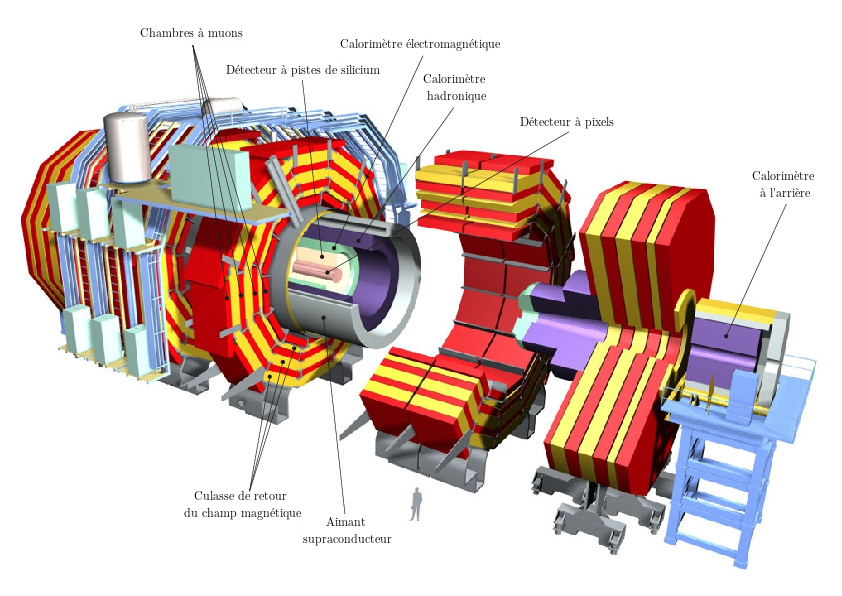
\includegraphics[width=0.8\textwidth]{CMS/cms.png}
	\caption{\label{cmsexploded}Vue éclatée du détecteur CMS.}
\end{sidewaysfigure}
